\chapter{State of the art}\label{ch:state-of-the-art}

In this chapter, the fundamental concepts and existing solutions related to the problem of
this dissertation are presented.
Section~\ref{sec:6g_charac} introduces 5G and 6G, addressing target performance requirements, emerging technologies, and envisioned applications.
It also briefly compares 5G and previous generations of mobile networks.
In Section~\ref{sec:5g_arch}, the main components and interfaces of the 5G architecture are presented and explained.
In Section~\ref{sec:RAN}, different RAN deployment approaches are explored and compared, including O-RAN. The O-RAN architecture and its specifications are presented with greater emphasis in Section~\ref{sec:ORAN}.
Section~\ref{sec:CV} presents an overview of state-of-the-art tools used for the detection and tracking using Computer Vision.
Section~\ref{sec:rel_work} describes different solutions leveraging video sensing for wireless networks.
Section~\ref{sec:CONVERGE} discusses the objectives and architecture of the CONVERGE project.
Finally, Section~\ref{sec:Summary_SOA} summarizes the content of this chapter.

\section{5G and 6G Characterization} \label{sec:6g_charac}
The evolution from 4G to 5G represented a substantial advancement in mobile communications standards, addressing the limitations posed by the surge in connected devices and emerging technologies like the Internet of Things (IoT) and augmented reality (AR). The demand for faster and more reliable connectivity motivated the development of 5G, introducing higher frequency bands, wider channel bandwidths, and advanced antenna designs~\cite{5G_apps}.

In the 6G paradigm, evolution is set to be even more transformative.
6G aims to surpass 5G in data rates, latency, and connectivity, as shown in Figure~\ref{fig:6g_capab}.
The 6G design effort has already begun.
The International Telecommunication Union (ITU) has advanced the development of 6G mobile technologies by publishing the framework for standards and radio interface technologies, known as Recommendation ITU-R M.2160-0~\cite{ITU_2160-0}, confirming the name for the next generation of IMT (“6G”) to be “IMT-2030”.
The ITU's document introduces the expected capabilities of 6G technology and envisioned usage scenarios.
This includes immersive communications, hyper-reliable and low-latency communications for industrial applications, enhanced ubiquitous connectivity, massive communications for IoT, and integration with artificial intelligence~\cite{6G_ITU}.
The use of terahertz frequency bands and the integration of artificial intelligence for network optimization and management are also envisioned~\cite{6G_ITU}.
Quantum communications, a concept not fully realized in previous generations, may become a reality in 6G, providing unprecedented security for wireless communications~\cite{6G_ITU}.

\begin{figure}[H]
    \centering
    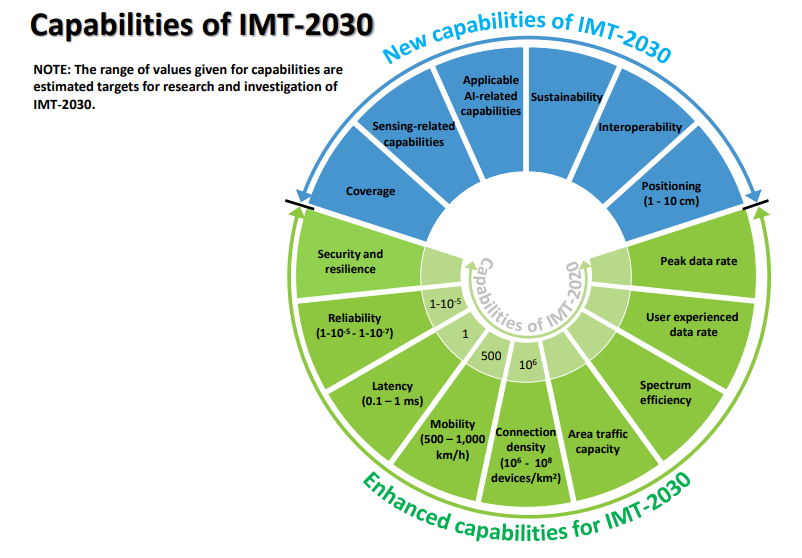
\includegraphics[width=0.8\linewidth]{figures/capabilities 6g}
    \caption[Capabilities of IMT-2030]{Capabilities of IMT-2030 \cite{ITU_2160-0}.}
    \label{fig:6g_capab}
\end{figure}

The proposed 6G applications include Unmanned Aerial Vehicle (UAV) networks, fully automated Vehicle-to-Everything (V2X), and holographic conferencing~\cite{6G_ITU}.
These applications were initially envisioned for 5G but were only partially realized, emphasizing their priority in 6G development~\cite{6G_ITU}.
The predicted usage scenarios are depicted in Figure~\ref{fig:6g_usage}.

5G networks have three main service categories that define the requirements and use cases for different types of applications.
6G is expected to extend those, depicted in Figure~\ref{fig:6g_usage}: Enhanced Mobile Broadband (eMBB), Massive Machine Type Communications (mMTC), and Ultra-Reliable and Low Latency Communications (URLLC), which are described as follows:.
\begin{itemize}
    \item \textbf{eMBB}: aims to provide a better user experience for mobile broadband services, such as video streaming, virtual and augmented reality, and online gaming.
    eMBB requires high data rates, high spectral efficiency, and wide coverage.
    \item \textbf{URLLC}: supports use cases that require strict quality of service levels, such as autonomous driving, remote surgery, and industrial automation.
    URLLC requires high reliability, low latency, and high availability.
    \item \textbf{mMTC}: enables various applications that collect and exchange data from sensors, meters, and machines, such as smart agriculture, smart city, and smart grid applications.
    mMTC requires high device density, low power consumption, and low data rates.
\end{itemize}

These three service categories are not mutually exclusive; some applications may require a combination.
For example, a smart factory may need eMBB for high-definition video surveillance, mMTC for monitoring and controlling machines, and URLLC for real-time feedback and coordination.

\begin{figure}[H]
    \centering
    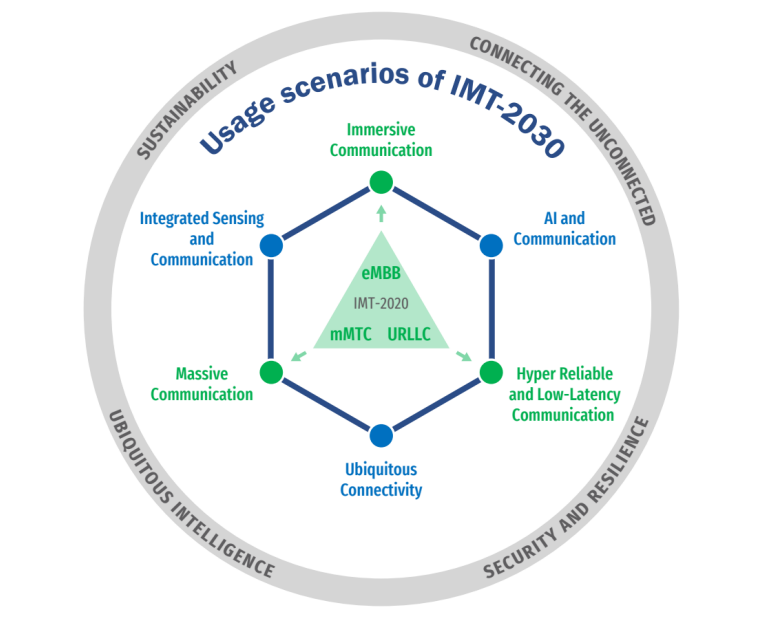
\includegraphics[width=0.5\linewidth]{figures/usage 6g}
    \caption[Usage scenarios and overarching aspects of IMT-2030]{Usage scenarios and overarching aspects of IMT-2030 \cite{ITU_2160-0}.}
    \label{fig:6g_usage}
\end{figure}

In 6G, progress is not only focused on enhancing data rates and connectivity.
The shift towards open-source frameworks is a pivotal aspect, driven by the recognition that collaborative, community-driven development accelerates the evolution of network technologies~\cite{6G_SOA}.
This open-source paradigm aims to create a more inclusive, adaptable ecosystem where diverse contributors shape the future of wireless communications~\cite{6G_SOA}.


\section{5G Architecture} \label{sec:5g_arch}

Considering the ongoing evolution and yet-to-be-fully-defined nature of the 6G architecture, this dissertation will utilize the established framework of 5G. The 3rd Generation Partnership Project (3GPP) stands behind the evolution of mobile communication standards~\cite{3GPP_about_us}.
The 5G New Radio (NR) architecture, a 3GPP standardization, embodies this commitment.
By embracing the principles of Software Defined Networking (SDN), 3GPP enhanced wireless communications into scalability and flexibility.
The strategic division of the control and data planes facilitates dynamic adaptability, empowering networks to respond to evolving demands and optimize resource utilization quickly.

The 3GPP model design maximizes interoperability with legacy infrastructure and equipment, promising an end-to-end ecosystem capable of supporting various use cases.
A high-level architecture of 5G NR is presented in Figure~\ref{fig:5G_arch}.

\begin{figure}[H]
    \centering
    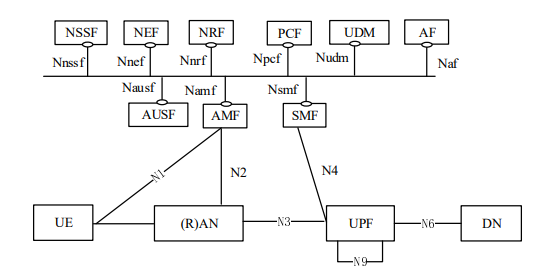
\includegraphics[width=0.7\linewidth]{figures/5g NR}
    \caption[High-level 5G NR Architecture]{High-level 5G NR Architecture \cite{ETSI_5G_NR}.}
    \label{fig:5G_arch}
\end{figure}

There are several relevant components in 5G NR, each playing a role in offering high-speed, low-latency connectivity for diverse applications and services.
The User Equipment (UE) is at the forefront, including smartphones, IoT devices, and user terminals connected to the 5G network.
The Radio Access Network (RAN) employs techniques, including Massive MIMO and beamforming, to optimize the performance of wireless communications established between UEs and the Core network.
It employs a base station, also called gNodeB (gNB).

Within the Core network, the Access and Mobility Management Function (AMF) oversees access and mobility, ensuring a seamless and dynamic user experience.
The Authentication Server Function (AUSF) guarantees secure user authentication, adding a layer of robustness to the network's security infrastructure.
The Network Slice Selection Function (NSSF) assists in selecting appropriate network slices based on service requirements, tailoring the network to specific needs.

Other components include the Network Exposure Function (NEF), the enabler for exposing network assets and services to external applications.
The Network Repository Function (NRF) maintains a repository of critical network information, contributing to the network's overall intelligence.
The Policy Control Function (PCF) manages policy enforcement and control, including Quality of Service (QoS) and network slicing policies that define the user experience.
The Unified Data Management (UDM) handles subscriber data.
The Application Function (AF) oversees application-specific functions, enriching the user experience with tailored capabilities.
Finally, the User Plane Function (UPF) manages user data traffic, and the Data Network (DN) allows the connection of the UPF to external data networks.
These entities ensure efficient resource utilization and enhance the network's capabilities.

\section{RAN Deployment Approaches} \label{sec:RAN}
The traditional deployment of RANs involves strategically placing base stations and network infrastructure to enable wireless communications between UEs and the Core network, using radio signals for wireless connectivity.

In the conventional RAN deployment model, the Base Band Unit (BBU) and Remote Radio Unit (RRU) are central entities.
The BBU manages the base station and ensures connectivity with the Core network, while the Remote Radio Head (RRH), connected to the base station's antenna, enables radio communication.
Figure~\ref{fig:rru_bbu} depicts this deployment approach.

\begin{figure}[H]
    \centering
    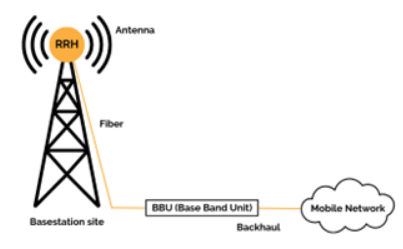
\includegraphics[width=0.5\linewidth]{figures/RRU_BBU}
    \caption[Traditional RAN deployment approach]{Traditional RAN deployment approach \cite{Trad_RAN}.}
    \label{fig:rru_bbu}
\end{figure}

Despite its widespread adoption, this approach faces several challenges, including concerns about achieving uniform coverage across diverse terrains, meeting the escalating demand for high data rates, and accommodating the increasing number of connected devices.

Network equipment providers typically design RAN implementations based on closed systems, lacking compatibility with equipment from other providers.
This limitation forces network operators to rely on solutions from a single equipment provider, abdicating flexibility and interoperability.
However, deploying and maintaining a network of physical base stations is a significant expense.
In addition, the potential for interference between adjacent cells poses challenges to spectrum efficiency and overall network performance, particularly as the number of deployed base stations increases.
Finally, adapting or expanding the network to meet growing user demands or technological advancements becomes a complex and time-consuming task within the traditional RAN deployment model.

Several solutions have emerged to address the challenges posed by traditional RAN deployments, offering enhanced flexibility, scalability, and efficiency.
These solutions are based on softwarization and virtualization, utilizing the principles of Network Function Virtualization (NFV) and SDN. An alternative solution is the implementation of Cloud RAN (cRAN). By centralizing the BBUs in cloud data centers, this architecture introduces a more dynamic and adaptable approach to RAN deployment, as shown in Figure~\ref{fig:cRAN}.
The data centers, interconnected with RRUs in base stations through fronthaul interfaces, host virtualized BBUs aggregated in a pool and executed on a single machine.
cRAN leverages Cloud computing principles to enhance scalability and resource optimization.
This setup offers advantages such as capacity load balancing and heightened signal processing capabilities.
However, C-RAN still faces the challenge of vendor lock-in, as systems and interfaces rely on proprietary implementations, which limits interoperability.

\begin{figure}[H]
    \centering
    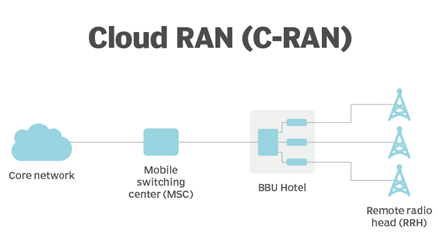
\includegraphics[width=0.5\linewidth]{figures/cRAN}
    \caption[cRAN deployment approach]{cRAN deployment approach \cite{cRAN}.}
    \label{fig:cRAN}
\end{figure}

Virtual RAN (VRAN) introduces a distinct approach for RAN deployment, leveraging NFV principles.
In contrast to cRAN, which centralizes baseband processing on proprietary hardware, VRAN considers a virtualized model.
This involves the replacement of specialized hardware with Commercial Off-the-shelf (COTS) hardware, providing a platform for deploying BBU nodes.
However, the interfaces between the RRU and the virtualized BBU remain closed, and the interoperability challenge is not fully addressed.


To address the interoperability challenge, the 3GPP has created a disaggregation of the gNB into a gNB Central Unit (gNB-CU) connected to one or more gNB Distributed Units (gNB-DUs) via the F1 interface, as depicted in Figure~\ref{fig:gnbdiss}.
This disaggregation offers a standardized alternative, providing a more interoperable solution.
The gNB-CU and gNB-DUs, while distributed, ensure effective communications through standardized interfaces, overcoming the closed interface limitations of traditional VRAN deployments.
This leads to compatibility between virtualized network functions from different vendors, promoting a more flexible and vendor-neutral RAN architecture.

\begin{figure}[H]
    \centering
    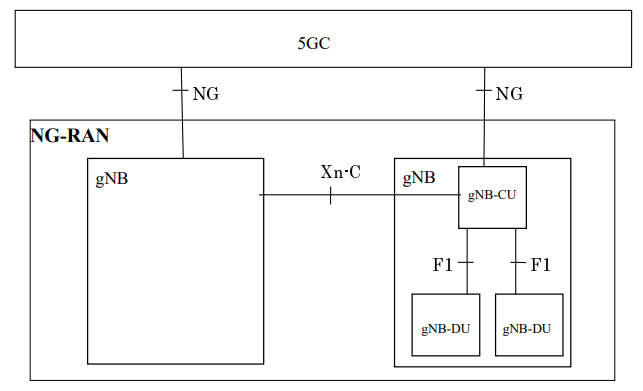
\includegraphics[width=0.6\linewidth]{figures/gnb_diss}
    \caption[Disaggregated gNB]{Disaggregated gNB \cite{gnb_diss}.}
    \label{fig:gnbdiss}
\end{figure}

The latest solution to these challenges is Open RAN (O-RAN). O-RAN represents a paradigm shift from traditional, closed RAN architectures, introducing openness and interoperability.
This approach uses the disaggregated gNB previously mentioned and virtualization through COTS. O-RAN's main principle is to provide standardized interfaces, fostering interoperability between equipment from diverse providers.
It promotes innovation and addresses the interoperability issues prevalent in closed systems.
By embracing O-RAN, network operators can choose components based on performance, cost, and targeted use cases.
This approach significantly reduces vendor lock-in, allowing for a more dynamic and cost-effective RAN deployment.
The following section focuses on O-RAN, central to this dissertation's solution.


\section{O-RAN}\label{sec:ORAN}
At the core of O-RAN's initiatives is the development of its reference architecture, depicted in Figure~\ref{fig:ORAN}, which defines open interfaces and specifications.
This section discusses the O-RAN architecture; it is divided into   Subsection~\ref{subsec:components} for the key components and Subsection~\ref{subsec:interfaces} for the interfaces of O-RAN\@.
 
\begin{figure}[H]
    \centering
    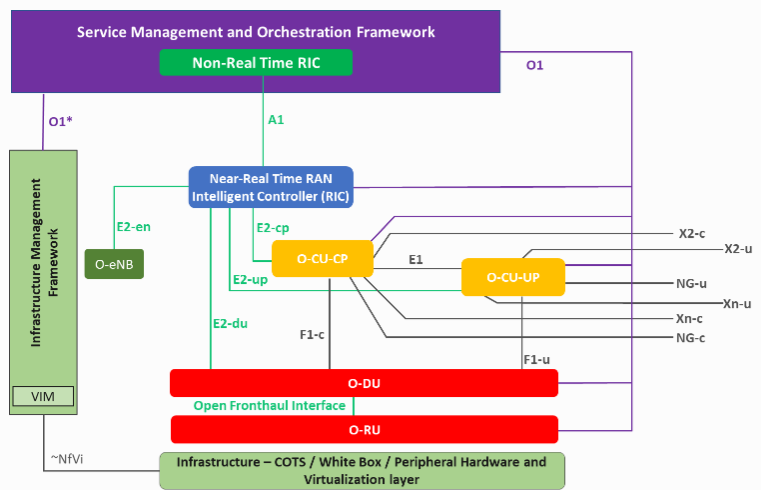
\includegraphics[width=0.6\linewidth]{figures/ORAN}
    \caption[O-RAN architecture overview]{O-RAN architecture overview \cite{ORAN-ARCH}.}
    \label{fig:ORAN}
\end{figure}

\subsection{O-RAN Components}\label{subsec:components}
The O-RAN architecture comprises several key components, each serving a specific function to enhance network performance and promote openness and interoperability.
The Centralized Unit Control Plane (O-CU-CP) and the Centralized Unit User Plane (O-CU-UP) are integral parts of the O-RAN architecture.
The O-CU-CP handles the centralized control plane functions, enabling efficient coordination and management of radio resources.
On the other hand, the O-CU-UP focuses on user plane functions, dealing with the processing and forwarding user data.
The O-CU-CP implements higher layers of the 3GPP protocol stack, such as the Radio Resource Control (RRC) layer, managing the connection life cycle.
The O-CU-UP also implements the higher layers of the 3GPP protocol stack.
However, it manages the Quality of Service (QoS) of the traffic flows and handles reordering packet duplication and encryption for the wireless interface.
They can both be deployed in the Cloud or at the Edge of the network and can communicate with multiple O-DUs and O-RUs.

The Distributed Unit (O-DU) decentralizes the baseband processing functions.
It collaborates with the Radio Unit (O-RU), responsible for radio frequency transmission and reception.
This separation of functions enhances scalability, allowing for more flexible and efficient resource allocation.
The O-DU implements the lower layers of the 3GPP protocol stack, such as the Radio Link Control (RLC) layer, the Medium Access Control (MAC) layer, and part of the physical layer.
It can be virtualized on servers at the Edge of the network, connecting to one or more O-RUs through the O-RAN Open Fronthaul interface.
The O-DU also interacts with the near-Real-Time Radio Intelligent Controller (Near-RT RIC) through the E2 interface, enabling data-driven closed-loop control and optimization of the RAN\@.

The O-RU implements the remaining part of the physical layer and the Radio Frequency (RF) components.
It is usually deployed close to the antennas, connecting to one or more O-DUs through the O-RAN Open Fronthaul interface.
The O-RU performs time-domain functionalities, such as precoding, Fast Fourier Transform (FFT), cyclic prefix addition/removal, and beamforming.

Near-RT RIC and Non-Real-Time (Non-RT) RIC introduce intelligence and automation into the O-RAN ecosystem.
The Near-RT RIC manages and controls the RAN at Near-real-time (10 ms to 1 s) time scale.
It is deployed at the Edge of the network, interacting with multiple O-DUs and O-CUs through the E2 interface.
The Near-RT RIC hosts multiple applications, called xApps, which implement custom logic for RAN optimization and control.
In contrast, the Non-RT RIC manages and controls the RAN at non-real-time (more than 1 s) time scale.
It is part of the Service Management and Orchestration (SMO) framework, complementing the Near-RT RIC for intelligent RAN operation and optimization.
The Non-RT RIC hosts multiple applications, called rApps, providing value-added services to support and facilitate RAN optimization and operations.

\subsection{O-RAN Interfaces} \label{subsec:interfaces}

The O-RAN architecture relies on multiple interfaces that enable seamless communications, control, and data exchange among diverse components of O-RAN. These open interfaces ensure interoperability, flexibility, and efficient orchestration within the RAN ecosystem.

One crucial interface is the E2 interface, which establishes a connection between the Near-RT RIC and the RAN nodes, including the Centralized Unit (CU) and Distributed Unit (DU). Through the E2 interface, the Near-RT RIC gains access to data from the RAN, enabling informed decision-making and facilitating the transmission of control actions and policies to optimize RAN performance.
The E2 interface supports various message types, such as subscription, indication, control, and policy, contributing to the dynamic adaptability of the RAN\@.

The A1 interface enables communications between the non-RT RIC and the Near-RT RIC. It is responsible for policy guidance and enrichment.
This interface allows the non-RT RIC to provide valuable insights and receive feedback and status reports from the Near-RT RIC. By supporting message types like policy type, policy instance, and service model, the A1 interface fosters cooperation between different RIC components, enhancing overall RAN intelligence.

The O1 interface connects the SMO framework and the RAN nodes (CU, DU, and RU). It empowers the SMO to perform essential functions, including configuration, fault management, performance monitoring, and security management of the RAN elements.
With support for various message types, such as configuration, fault, performance, and security management messages, the O1 interface ensures efficient and centralized management of the RAN\@.

The O-RAN Open Fronthaul interface establishes a critical link between the DU and the RU, facilitating the exchange of user and control plane data.
Additionally, it enables the DU to configure and manage the RU functionalities.
Built on top of the eCPRI and IEEE 1914.3 standards, this interface supports different message types, including user plane, control plane, synchronization plane, and management plane messages, ensuring a flow of information between the DU and RU\@.

Finally, the O2 interface serves as a bridge between the SMO and the O-Cloud.
This interface empowers the SMO to orchestrate and manage virtualized network functions hosted on the O-Cloud platform.
With support for diverse message types, including inventory, monitoring, provisioning, fault tolerance, and update messages, the O2 interface facilitates the efficient coordination and deployment of virtualized network functions.

The O-RAN architecture promotes cooperation and innovation across the ecosystem, allowing network operators to seamlessly integrate components from different vendors.
This open and interoperable approach fosters competition, accelerates technological evolution, and empowers operators to tailor their networks according to specific requirements.
The O-RAN Alliance's role in standardization efforts is essential in guaranteeing consistency and compatibility across the diverse elements of the O-RAN architecture.


\subsubsection{E2 Interface}\label{subsubsec:protocols}
The E2 interface connects the Near-RT RIC to the E2 nodes.
The interaction between these entities is defined by the E2 Service Model (E2SM).
Each E2SM model defines a service that a RAN function can perform.
The basic actions are: report, insert, control and policy.
Each of these is transported through E2 Application Protocol (E2AP) procedures.

For instance, a report contains information from the E2 nodes to the RIC/xApps.
An xApp sends an E2AP subscription to request a report.
The E2SM specifies the types of reports that can be sent and the events that trigger them.
Then, the RAN function sends an E2SM report transported through an E2AP Indication Message.

Thus, the E2 interface uses the E2 Application Protocol (E2AP) to handle signaling and control procedures.
E2 Service Models (E2SMs) define the specific application-level data and control exchanges, enabling the Near-RT RIC to efficiently interact with and manage RAN functions in a standardized and customizable manner.
The protocol stack of the E2 interface is depicted in Figure~\ref{fig:E2_stack}.

\begin{figure}[H]
    \centering
    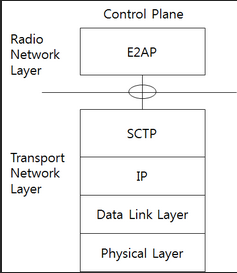
\includegraphics[width=0.3\linewidth]{figures/E2_stack}
    \caption[E2 protocol stack]{E2 protocol stack \cite{E2GAP}.}
    \label{fig:E2_stack}
\end{figure}

The E2AP messages are encoded in Abstract Syntax Notation One (ASN.1) Basic Packed Encoding Rules (BASIC-PER) Aligned Variant.
The encoding rules are defined in ITU-T Rec.
C.691~\cite{ITU_T_C691}.
ASN.1 is a standard interface description language for defining data structures that can be serialized and deserialized in a cross-platform way.

The E2AP services are categorized into two groups: RIC Functional Procedures and Global Procedures.
RIC Functional Procedures include actions used to pass application-specific messages between Near-RT RIC applications and a target RAN function in an E2 node.
The RIC Functional Procedures are designed to handle application-specific messaging.
These procedures facilitate the communication between Near-RT RIC applications and a target RAN function within an E2 node.
They include:

\begin{itemize}
\item RIC Subscription: Enables the Near-RT RIC to subscribe to specific events or data from the RAN functions.
\item RIC Indication: Allows the RAN functions to send reports or indications to the Near-RT RIC based on the subscribed events.
\item RIC Control: Permits the Near-RT RIC to send control messages to manage and influence the behavior of the RAN functions.
\end{itemize}
These functional procedures ensure adaptive and real-time management of the RAN, providing mechanisms for monitoring, reporting, and controlling various aspects of the network.

The Global Procedures are utilized for essential operations for the overall management and maintenance of the E2 interface.
They include:

\begin{itemize}
\item E2 Setup: Establishes the initial configuration and setup of the E2 interface between the Near-RT RIC and the E2 nodes.
\item E2 Configuration Update: Updates the configuration parameters of the E2 interface as required by changes in the network or operational policies.
\item E2 Reset: Handles the reset operations to recover from error conditions or to reinitialize the E2 interface.
\end{itemize}
These global procedures ensure that the E2 interface is capable of handling various network scenarios and requirements.



\section{Computer Vision}\label{sec:CV}

CV, a branch of artificial intelligence, enables machines to interpret and make decisions based on visual data, involving the understanding and analyzing of images and videos.
Object detection and tracking are tasks of CV, allowing machines to identify, locate, and monitor specific objects within visual content while facilitating recognition and comprehension of real-world scenarios.CV is used in various domains.
In autonomous vehicles, object detection and tracking tasks ensure safe navigation by identifying pedestrians, vehicles, and obstacles.
Retail uses CV for automated checkout and inventory management, while security systems employ it for real-time monitoring and tracking of suspicious activities.
Augmented reality relies on CV to seamlessly integrate virtual elements into the real world.

In mobile networks, object detection and tracking may play a key role in optimizing network performance.
They may allow for analyzing user behavior patterns, helping telecom providers to enhance coverage and capacity in areas with high user density.
In the context of 5G networks, obstacle-aware networks utilize object detection and tracking to improve communications efficiency and reliability in the presence of obstacles.
Object detection and tracking allow identifying and categorizing obstacles while enabling dynamic adjustments of network parameters for optimized signal strength and connectivity.
Integrating vision-based capabilities in 5G systems paves the way to enable proactive responses to environmental changes, mitigating signal blockage and enhancing overall communications quality.
Overall, object detection and tracking contribute to improved network performance, efficient maintenance processes, and an enhanced user experience in the mobile telecom sector.

This section is further divided into three sections.
Section~\ref{subsec:detect} discusses the state-of-the-art detection models.
Section~\ref{subsec:track} discusses the tracking solutions.
Finally, Section~\ref{subsec:open_tools} evaluates the existing open-source tools, their applicability, and their relevance to the specific challenges addressed in this dissertation.

\subsection{Detection models}\label{subsec:detect}

Object detection models are essential in locating and classifying objects within images, utilizing bounding boxes and labels.
Generic object detectors, foundational in CV, exist in two main types: two-stage and one-stage detectors.
Two-stage detectors, exemplified by Faster Region-based Convolutional Neural Network (Faster R-CNN)~\cite{FasterRCNN}, lie in a traditional approach of proposing regions of interest (RoIs) before classifying and refining them.
This method prioritizes accuracy but may have longer processing times.
On the other hand, one-stage detectors, such as You Only Look Once (YOLO)~\cite{YOLO} and Single Shot MultiBox Detector (SSD)~\cite{SSD}, optimize the process by predicting bounding boxes and class probabilities in a single pass, prioritizing real-time performance.
These detectors are versatile and crucial in applications like image recognition and can be applied to diverse scenarios.
Figure~\ref{fig:1vs2} depicts the differences in the architecture of one-stage and two-stage detectors.

\begin{figure}[H]
    \centering
    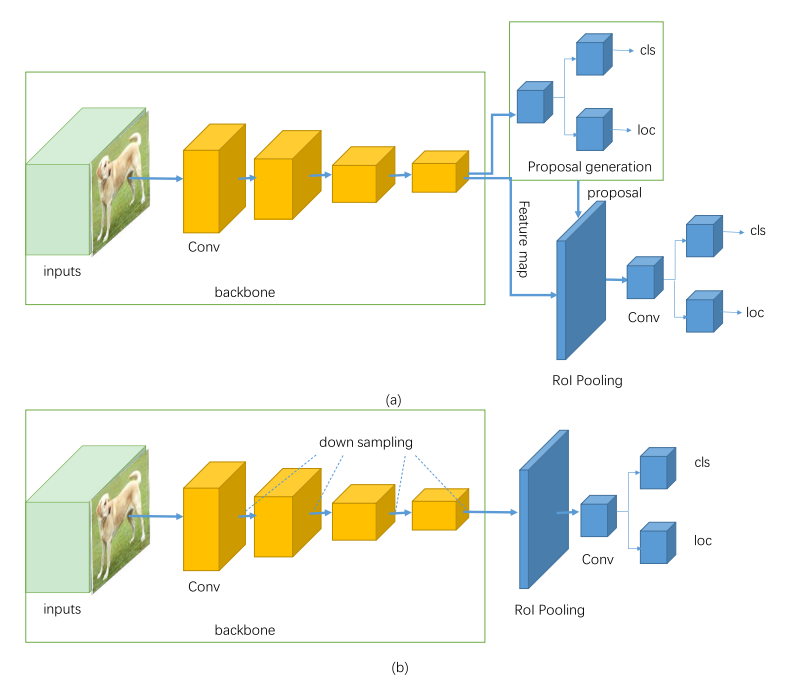
\includegraphics[width=0.6\linewidth]{figures/single vs two}
    \caption[Two stages vs. single stage detector architecture]{Two stages vs. single stage detector architecture. (a) Exhibits the basic architecture of two-stage detectors, and (b) shows the basic architecture of one-stage detectors \cite{1vs2}.}
    \label{fig:1vs2}
\end{figure}

In the case of two-stage detectors, as depicted in Figure~\ref{fig:1vs2} (a), the architecture involves a region proposal network (RPN) in the initial phase.
The RPN takes input images and generates region proposals or bounding boxes that are likely to contain objects of interest.
These proposals are then fed into a classifier and regressor for further processing.
The classifier determines the object's class within each proposed region, while the regressor refines the coordinates of the bounding boxes.
This two-stage approach allows for systematic and staged input processing, providing a more detailed analysis that often leads to improved accuracy.

Conversely, Figure~\ref{fig:1vs2} (b) illustrates the basic architecture of one-stage detectors.
In this case, the detector predicts bounding boxes directly from the input images without needing a separate region proposal network.
The architecture involves a series of convolutional layers forming a backbone network.
The yellow cubes represent these convolutional layers, organized into blocks with the same resolution.
Due to down-sampling operations after each block, the subsequent cubes gradually decrease in size.
The thick blue cubes, consisting of convolutional layers, handle the final prediction, including object classification and bounding box regression.
Notably, the flat blue cube represents the RoI pooling layer, which generates feature maps for objects of the same size.
This one-stage approach prioritizes simplicity and speed, making it particularly efficient for real-time applications, though it may face challenges in accurately detecting small or occluded objects.


The decision between single-shot and two-shot detectors involves balancing speed, accuracy, and complexity.
Single-shot detectors like YOLOv3~\cite{YOLOv3} process images in a single pass, prioritizing speed and simplicity without a separate RPN. This means that single-shot detectors employ one module comprising both tasks instead of having separate modules in the architecture for the RPN and the Classification and Regression Heads.
For this reason, they are simple to train and deploy but may sacrifice accuracy, especially for small or occluded objects.
In contrast, two-shot detectors like Faster R-CNN improve accuracy and reliability by employing a region proposal network and a separate classification network.
They handle complex scenes and small objects efficiently but are slower, more complex, and computationally intensive.
The choice between the two detectors hinges on the application's specific needs, requiring the consideration of trade-offs between speed and accuracy.


\subsection{Tracking models}\label{subsec:track}

Regarding deep learning-based object tracking, the methods can be classified into three distinct categories, each leveraging deep neural networks for enhanced tracking performance.
Firstly, deep network features-based methods enhance tracking by utilizing semantic features extracted from deep Convolutional Neural Networks (CNNs).
These methods employ various approaches to learn affinities between detections and track-lets, incorporating techniques such as multiple hypothesis tracking, Siamese networks, or optical flow features.
An example of this is the Siam R-CNN~\cite{siam}.
It has applications in scenarios where precise and robust object tracking is required, including in surveillance systems for accurate monitoring of individuals or objects.
However, the computational complexity of Siamese-based methods may make them less suitable for real-time applications on resource-constrained devices within mobile networks.
Another example in this category is Simple Online and Real-time Tracking with a Deep Association Metric (Deep SORT)\cite{DeepSORT}.
Deep SORT extends the capabilities of the SORT algorithm~\cite{SORT} by integrating deep learning techniques, specifically using deep features for association and tracking.
This extension enhances the algorithm's ability to handle challenging scenarios such as occlusions and varying object appearances, making it valuable in real-time scenarios, including traffic monitoring or event surveillance within mobile networks.

Secondly, deep network embedding-based methods integrate deep CNNs as the central component of the tracking framework.
These methods adopt different learning tasks, including discriminative, metric, or generative learning, to estimate parameters or distances for matching detections and track-lets.
The discriminative Correlation Filter (DCF) trackers, such as the Kernelized Correlation Filter (KCF)~\cite{KCF}, represent an influential category.
These trackers leverage deep CNNs as integral components, employing discriminative learning tasks to estimate parameters for matching detections and track-lets.
Their application extends to scenarios where a balance between accuracy and real-time performance is essential, including in video analysis for content creation, in which tracking objects efficiently contributes to the overall editing process.

Finally, end-to-end deep network learning-based methods take a direct approach by using deep networks to output tracking results without relying on intermediate steps.
These methods leverage diverse architectures, such as Recurrent Neural Networks (RNNs), Long Short-Term Memory Networks (LSTMs), and attention mechanisms, to model the temporal dependencies and dynamics of the tracked objects.
Algorithms like LSTM trackers and Attention-based trackers demonstrate the effectiveness of direct end-to-end approaches.
LSTMs demonstrate effectiveness in applications requiring temporal understanding, benefiting video-based tasks such as action recognition or gesture tracking.
However, the resource-intensive nature of LSTMs may impact real-time performance, making them less suitable for deployment in mobile networks with limited computational resources.
On the other hand, Attention-based trackers, exemplified by algorithms like ATOM, offer efficient solutions for applications demanding real-time visual attention, such as augmented reality experiences on mobile devices.

While concepts of CV are discussed in this subsection, it is important to note that the specific exploration of dedicated object detection algorithms tailored for distinct applications will not be covered in this context.
The focus remains on the fundamental principles, applications, and the broader scope of object detection and tracking within the generic object detectors.
Specialized algorithms designed for specific applications, while integral to the field, ensure in-depth discussions tailored to their unique contexts and use cases, which may extend beyond the scope of this work.
More extensive research on state-of-the-art object detection and tracking can be found at~\cite{obj_detec_SOA}.

\subsection{Open-source Tools}\label{subsec:open_tools}
In object detection and tracking, open-source tools are essential in providing accessible and adaptable solutions.
Integrating these tools into a gNB based on the O-RAN architecture in real-time applications requires careful consideration of speed, accuracy, and compatibility.
Two notable tools mentioned previously stand out for their effectiveness: YOLO and BoT-SORT\@.

YOLO\cite{YOLO} has gained attention in both academic research and practical applications.
YOLO's one-shot detection approach is foundational to its success, as it processes the entire image in a single pass.
This approach is particularly advantageous for applications demanding low latency, making it a compelling choice for integration within an O-RAN architecture.
Table~\ref{tab:yolo_performance} presents a comparison made in~\cite{YOLO_compare} based on mean Average Precision (mAP) and frames-per-second (fps) between different YOLO models to run a video on CPU and GPU, proving the evolution of the algorithm.

The mAP summarizes the classification performance of the object detection model across different categories, while the fps assesses the real-time performance of a model.

\begin{table}[H]
    \caption[Performance Metrics of Various YOLO Versions]{Performance Metrics of Various YOLO Versions \cite{YOLO_compare}.}
    \label{tab:yolo_performance}
    \centering
    \begin{tabular}{|l|l|l|l|l|l|}
        \hline
        Versions & mAP & CPU fps & GPU fps & CPU time (s) & GPU time (s) \\ \hline
        YOLOv3 & 33.2 & 2.88 & 37 & 324.539 & 14.625 \\
        YOLOv4 & 57.8 & 1.21 & 28.9 & 568.484 & 16.458 \\
        YOLOv4-tiny & 38.1 & 18.46 & 65.8 & 46.751 & 13.351 \\
        YOLOv5-nano & 28.0 & 6 & 40 & 87.168 & 15.536 \\
        YOLOvS-small & 37.4 & 4 & 36 & 152.821 & 18.187 \\
        YOLOv6-nano & 35.9 & 5.4 & 110.7 & 103.253 & 16.551 \\
        YOLOv6-small & 43.5 & 2.7 & 72.8 & 289.838 & 18.911 \\
        YOLOv6-tiny & 40.3 & 4.2 & 80.9 & 196.117 & 18.078 \\
        YOLOv7 & 66.7 & 0.76 & 42 & 970.85 & 16.075 \\
        YOLOv7-tiny & 53.4 & 3 & 50 & 201.78 & 12.955 \\ \hline
    \end{tabular}
\end{table}


Academic research has consistently recognized YOLO for its contributions to the CV field.
The original YOLO paper~\cite{YOLO} introduced a new approach to object detection, achieving remarkable accuracy and speed.
Since then, the YOLO architecture has undergone several iterations, each bringing improvements in terms of performance and usability.

\begin{figure}[H]
    \centering
    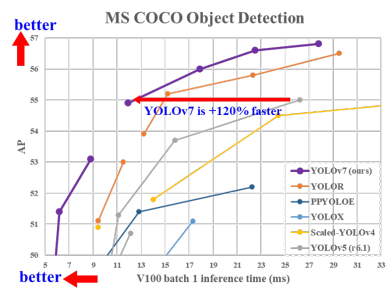
\includegraphics[width=0.6\linewidth]{figures/yolov7}
    \caption[Comparison between real-time object detectors]{Comparison between real-time object detectors \cite{yolov7}.}
    \label{fig:yolov7}
\end{figure}

One notable aspect of YOLO is its usability.
The architecture is designed to be accessible, making it easier for researchers and developers to implement and experiment with object detection.
The availability of pre-trained models further enhances the user experience, allowing practitioners to leverage the power of YOLO without an extensive background in deep learning.

The recent evolution of YOLO, including contributions from the Ultralytics~\cite{ultralytics_docs} team, has further improved its performance.
Ultralytics, a prominent contributor to YOLO's development, focuses on optimizing and advancing the capabilities of YOLO for real-world applications.
Their efforts have resulted in performance improvements, enhanced training capabilities, and a user-friendly interface, making YOLO even more attractive for applications demanding real-time object detection, such as those encountered in O-RAN architectures.
Figure~\ref{fig:yolov7} compares real-time object detectors.
Notice that, in the MS COCO dataset~\cite{COCO}, the algorithm that performs best is YOLOv7.

While all categories of object tracking methods presented in Section~\ref{subsec:track} can potentially be employed for Multiple Object Tracking, deep network features-based approach are presented herein.
SORT, a representative method in this category, is designed for efficient tracking by primarily relying on basic motion and position information to link detections across frames.
Although effective under ideal conditions, SORT may struggle with challenges like appearance variations and occlusions, due to its simplicity.

In response to these limitations, Bag of tricks for SORT based methods (BoT-SORT)\cite{botsort} has been developed.
BoT-SORT uses semantic features extracted from deep CNNs, which increases proficiency in distinguishing between different classes of obstacles, such as vehicles and pedestrians, even in occlusions scenarios and varying appearances.
This capability enables BoT-SORT to balance speed and accuracy, which makes it suitable for real-time tracking applications.


\begin{figure}[H]
    \centering
    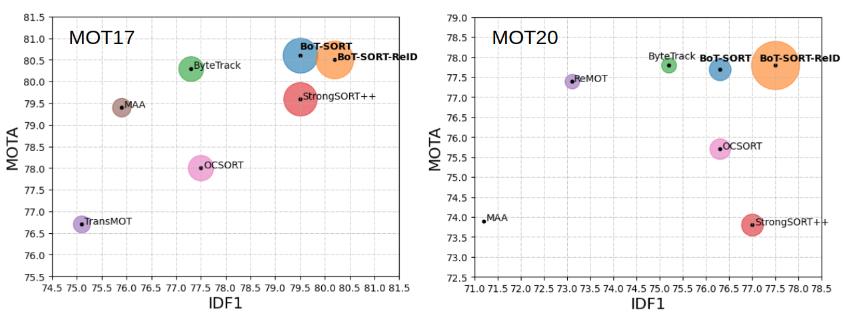
\includegraphics[width=0.8\linewidth]{figures/botsort}
    \caption[Comparison of state-of-the-art trackers in the MOT17 and MOT20]{ Comparison of state-of-the-art trackers in the MOT17 and MOT20 \cite{botsort}. Notice that BoT-SORT's models perform well in both challenges when compared to other models, as they are seen in the top right corner indicated by high MOTA and IDF1.}
    \label{fig:botsort}
\end{figure}

Figure~\ref{fig:botsort} compares trackers participating in the MOT17 and MOT20 challenges, highlighting the significant performance of BoT-SORT. The positioning of each tracker on the plot reflects its performance in terms of identification F1 Score (IDF1) on the horizontal axis and Multiple Object Tracking Accuracy (MOTA) on the vertical axis.
The circle's radius around each point indicates its Higher Order Tracking Accuracy (HOTA) score.

The IDF1 measures the accuracy of identity assignments in tracking results, encompassing precision and recall of identity associations.
A higher IDF1 score indicates a better ability to correctly associate detections with existing tracks while maintaining object identities over time.
For MOTA, \ref{fig:botsort} offers an overall assessment of tracking accuracy, considering various error sources such as false positives, false negatives, and identity switches.
A higher MOTA score indicates superior tracking accuracy, by penalizing tracking errors like missing detections and incorrect associations.
HOTA extends the evaluation beyond MOTA by incorporating additional information about the quality of track fragments.
 It considers the completeness, correctness, and assignment ambiguity of track fragments, providing a more nuanced evaluation of tracking performance.

The scores achieved by BoT-SORT demonstrate its effectiveness in accurately associating detections with tracks, maintaining object identities, and producing high-quality track fragments, making it a compelling choice for multiple object tracking tasks.

As presented in~\cite{botsort}, BoT-SORT presents a 6.6 Frames Per Second (FPS) score.
Considering the indoor scenario, this processing speed offers acceptable results for the intended application.
In indoor environments, where the movement of objects is typically constrained and relatively slow compared to outdoor scenarios, BoT-SORT should perform well.
This metric ensures that it can maintain real-time tracking capabilities in dynamic indoor environments.

The combination of acceptable performance metrics and a satisfactory FPS demonstrates the viability of BoT-SORT for indoor multiple object tracking applications.
It indicates that BoT-SORT can reliably track objects in real-time indoor scenarios accurately.

Regarding implementation, BoT-SORT is one of the supported trackers within the Ultralytics YOLO framework.
This choice offers benefits for object-tracking applications.
BoT-SORT's integration with YOLO ensures improved tracking accuracy, efficient real-time processing, and seamless object ID management, facilitating detailed analytics and monitoring in video streams.
Using BoT-SORT with Ultralytics' Python API enables quick deployment of tracking solutions.

The selection of YOLO and BoT-SORT is justified by their strengths in speed, accuracy, and adaptability to real-time applications.
Their integration into a video-based gNB within an O-RAN architecture aligns with the objective of efficient and reliable object detection and tracking in wireless communications networks.



\section{Related Work}\label{sec:rel_work}
In recent developments, a limited number of publications are exploring the integration of CV to enhance mobile networks, particularly within the framework of O-RAN\@.

In~\cite{Block_predict}, a machine learning framework is proposed to enable proactivity in wireless networks, leveraging visual data captured by video cameras at base stations.
The focus is on anticipating future blockages and facilitating user hand-offs in advance.
The proposed two-component deep learning architecture, using YOLOv3~\cite{YOLOv3}, incorporates bimodal data, employing visual and radio information to predict blockages proactively and execute seamless user hand-offs.
The results demonstrate the architecture's efficacy in accurately detecting blockages through experimentation, enhancing reliability, and reducing latency in the wireless network.
The system model considers a small-cell mmWave base station equipped with a uniform linear array and an RGB camera.
The channel considers a geometric mmWave model with L clusters, and the authors provide a mathematical formulation for modeling signal blockage while defining LoS and NLoS channels.
Moreover, they propose a future exploration based on the investigation of radar-based detection approaches to pinpoint the location of users who are served post-blockage.
This approach holds the potential for predicting blockages in real network environments with multiple users.
The proposed approach may be integrated with the O-RAN architecture, envisioning the implementation of the CU at the Near-RT RIC. This approach introduces potential enhancements to wireless networks' reliability and predictive capabilities.

A similar approach is presented in~\cite{Block_predict2}.
The authors employ CV to address challenges in mmWave wireless communications systems, specifically focusing on beam selection and blockage prediction.
Employing a synergy between CV and deep learning tools, the study proposes an approach for predicting mmWave beams and blockages directly from RGB images captured by cameras and sub-6GHz channels.
It eliminates the need for explicit channel knowledge or beam training.
Two deep learning-based solutions are proposed, anchored in deep convolutional networks and transfer learning, with a foundational reliance on the 18-layer Residual Network (ResNet-18).
This ResNet-18 model is tailored for beam prediction, treating the task as an image classification challenge while mapping images to beam indices from a codebook.
Simultaneously, another ResNet-18 model, equipped with a customized fully connected layer, performs user detection as a binary classification task, contributing to determining link status based on user detection results and sub-6GHz channel information.
The proposed approach shows the potential of CV and deep learning to revolutionize mmWave system capabilities, providing an innovative solution to address wireless communications challenges.

In~\cite{CVAided}, a real-world evaluation is presented leveraging visual data and machine learning techniques to predict mmWave dynamic link blockages proactively before they occur.
Proactive prediction of LoS link blockages enables mmWave/sub-THz networks to implement preemptive network management actions, such as proactive beam switching and hand-off, prior to link failures.
Such measures can significantly enhance network reliability, reduce latency and maximize the efficient utilization of wireless resources.
The study assesses the practical viability of this approach, by developing a Computer Vision-based solution that processes visual data captured by a video camera installed at the infrastructure node.
Additionally, the viability of their proposed solution is investigated using the DeepSense 6G~\cite{deepsense} dataset, which encompasses multi-modal sensing and communications data.
The results highlight the promising potential of integrating CV techniques in communications networks to mitigate link blockages and enhance network performance.

These works are part of a research group that developed DeepSense6G~\cite{deepsense}, a real-world multimodal sensing and communications dataset.
This dataset comprehends several scenarios utilizing various sensing approaches such as RGB cameras, radar, and LiDAR, including applications in beam prediction, blockage prediction and positioning.
DeepSense6G is designed to facilitate research in multimodal sensing and wireless communications, offering data that supports the development and evaluation of advanced algorithms.


In addition to DeepSense6G, there are other multimodal datasets that cater to different needs of the research community.
For instance, the Vision-Wireless (ViWi) dataset~\cite{ViWi} includes synchronized multimodal data from cameras, LiDAR, and wireless sensors, facilitating research in beamforming, user localization, and blockage prediction.
The ViWi dataset utilizes advanced 3D modeling and ray-tracing software to generate high-fidelity synthetic data, ensuring that both visual and wireless data samples are accurately represented for the same scenes.
By providing information based on both visual and wireless data, the ViWi dataset enables researchers to develop and validate algorithms that exploit the synergy between these modalities, leading to more robust and efficient communication systems.
The ViWi dataset is parametric, systematic, and scalable, making it possible to generate training and testing datasets and a common ground for assessing the quality of different machine learning-powered solutions.

Another reference dataset is the Synthesia of Machines~\cite{Synthesia}.
This dataset leverages advanced simulation techniques to generate multimodal data, including visual, audio, and sensory information.
The Synthesia of Machines dataset is particularly useful for training machine learning models in environments where collecting real-world data is challenging or impractical.
By providing high-quality synthetic data, this dataset helps researchers overcome the limitations of real-world data collection, allowing for the development and testing of algorithms in a controlled and scalable manner.
Synthetic data also facilitates exploring a wide range of scenarios and conditions, enhancing the robustness and generalizability of machine learning models.
ViWi and Synthesia of Machines leverage simulation to provide data environments for algorithm development and testing.

While the presented datasets enable significant advancements in multimodal sensing and have facilitated breakthroughs in various research areas, they still need to integrate with the ongoing efforts in the O-RAN architecture.

In the context of O-RAN deployments,~\cite{xApps} introduces OpenRAN Gym, a framework tailored for data-driven experimentation within the OpenRAN ecosystem, focusing on intelligent closed-loop control.
OpenRAN Gym enables the development, training, and testing of xApps, data-driven applications specifically designed for the near-RT RIC. The xApp design process integrates service models for communications with RAN nodes over the E2 interface, incorporating data-driven logic units hosting AI/ML models for RAN inference and control.
The framework's capabilities are exemplified through a compelling use case, considering an xApp that jointly manages scheduling and slicing functionalities of base stations based on real-time RAN data.
Rigorous testing on the Colosseum wireless network emulator, featuring seven base stations and forty-two users, highlights xApp's adaptability to diverse traffic scenarios.
The results emphasize the advantages of online fine-tuning, showcasing improved performance and generalization.
OpenRAN Gym's contribution lies in its potential to revolutionize intelligent closed-loop RAN control through the innovative development and application of xApps.
For these reasons,~\cite{xApps} is an important reference for best practices integrating object detection algorithms with the O-RAN architecture.

Regarding mobile gNBs, the goals of this dissertation are aligned with those achieved in ~\cite{maia2022control} and ~\cite{queiros2023autonomous}.
\cite{maia2022control} focuses on developing a private standalone on-demand 5G network, utilizing a 5G gNB carried by a mobile robotic platform.
The employed setup provides connectivity for 5G UEs.
It incorporates an On-Demand Mobility Management Function (ODMMF) for monitoring radio conditions of served UEs and remotely controlling the mobile robotic platform in real-time using its video cameras.
\cite{queiros2023autonomous}, on the other hand, focuses on deploying a private Standalone 5G Network with a mobile RAN employing the O-RAN architecture.
This approach leverages the standards and specifications proposed by the O-RAN Alliance to create open, interoperable networks based on independent virtualized components connected through standardized open interfaces.
The mobile RAN consists of a 5G gNB carried by a Mobile Robotic Platform capable of autonomous positioning.
The solution employs a novel Mobility Management xApp, which autonomously collects metrics from the RAN, analyzes them, and uses an algorithm to determine and control the placement of the mobile RAN to optimize connection quality between UEs and the gNB.
This demonstrates the potential of the O-RAN architecture to facilitate the deployment of multi-vendor components and enhance the flexibility and efficiency of 5G networks.
While these work are essential for the evolution of 5G networks and O-RAN, they do not integrate CV\@.

In summary, recent works have explored using CV and Machine Learning techniques to proactively predict dynamic link blockages in wireless networks, achieving high accuracy in blockage detection and showcasing the potential of CV and deep learning to enhance mmWave system capabilities.
Despite significant progress driven by the development of datasets in this field, further integration of these resources with the O-RAN architecture is necessary.
Such integration may enable new potentials in wireless communications, improving the efficiency of various applications.
To the best of our knowledge, there is a gap in the existing literature regarding solutions focused on integrating vision-based information with the O-RAN architecture, presenting an opportunity for contributions to O-RAN networks.



\section{CONVERGE project}\label{sec:CONVERGE}

The dissertation is aligned with the CONVERGE research project led by the Centre for
Telecommunications and Multimedia (CTM) of INESC TEC. CONVERGE aims at creating a
toolset that seamlessly integrates radio, CV, and sensing-based technologies,
embracing the motto \("\)view-to-communicate and communicate-to-view\("\)~\cite{converge_site}.

Figure~\ref{fig:chamber_converge} depicts the toolset to be deployed.
Four tools will be developed: Vision-aided Large Intelligent Surface, Vision-aided base station, Vision-radio simulator and 3D environment modeler, and Machine Learning (ML) algorithms.
Each of these tools aims to address specific research questions.
Given the objectives of the dissertation, the target tool to be understood and addressed is the Vision-aided base station.
While it will not be developed, only fed with relevant obstacle information, it is essential to comprehend its functionality.
It should enable communications with mobile terminals relating to beamforming, multi-user access, and opportunistic scheduling using video camera information.

\begin{figure}[H]
    \centering
    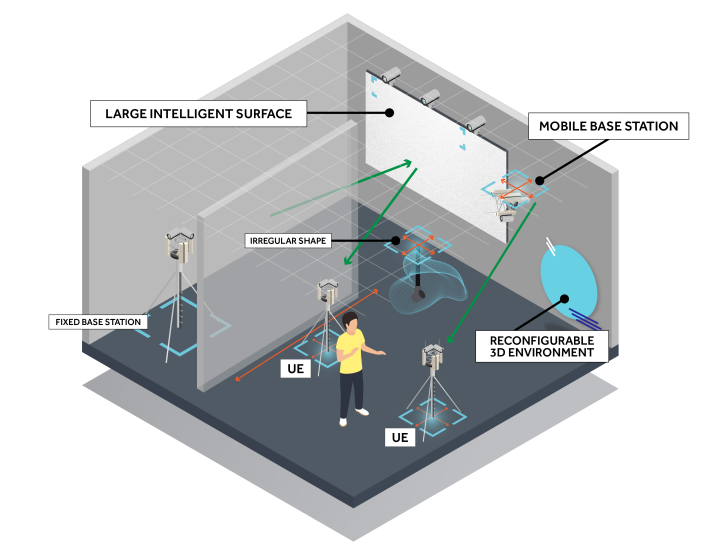
\includegraphics[width=0.7\linewidth]{figures/chamber_converge}
    \caption[Proposed vision-radio experimental chamber of the CONVERGE project]{Proposed vision-radio experimental chamber of the CONVERGE project \cite{converge2023_usecases}.}
    \label{fig:chamber_converge}
\end{figure}



Some of the questions mentioned in~\cite{converge2023_usecases} to be addressed by the project include:

\begin{itemize}
    \item How to detect the location of obstacles to signal propagation, interfering terminals, and terminals served by the vision-aided mobile base station?
    \item How does incorporating visual information impact the Quality of Experience (QoE) for UEs in terms of throughput, latency, and reliability?
    \item Which techniques are better suited to enable dynamic, collaborative tracking by incorporating information from multiple base stations or cameras within a network under variable environmental conditions or UE behavior?
\end{itemize}

Given this scope, understanding the CONVERGE project’s architecture is required.
It is
structured around three fundamental building blocks: the CONVERGE Chamber, the CONVERGE Core, and the CONVERGE Simulator, as illustrated in Figure~\ref{fig:converge_arch}.
This architectural division separates the physical infrastructure (the CONVERGE Chamber), the simulation infrastructure, the user interface, and the network and control functions, datasets,
and Machine Learning models (the CONVERGE Core).

\begin{figure}[H]
    \centering
    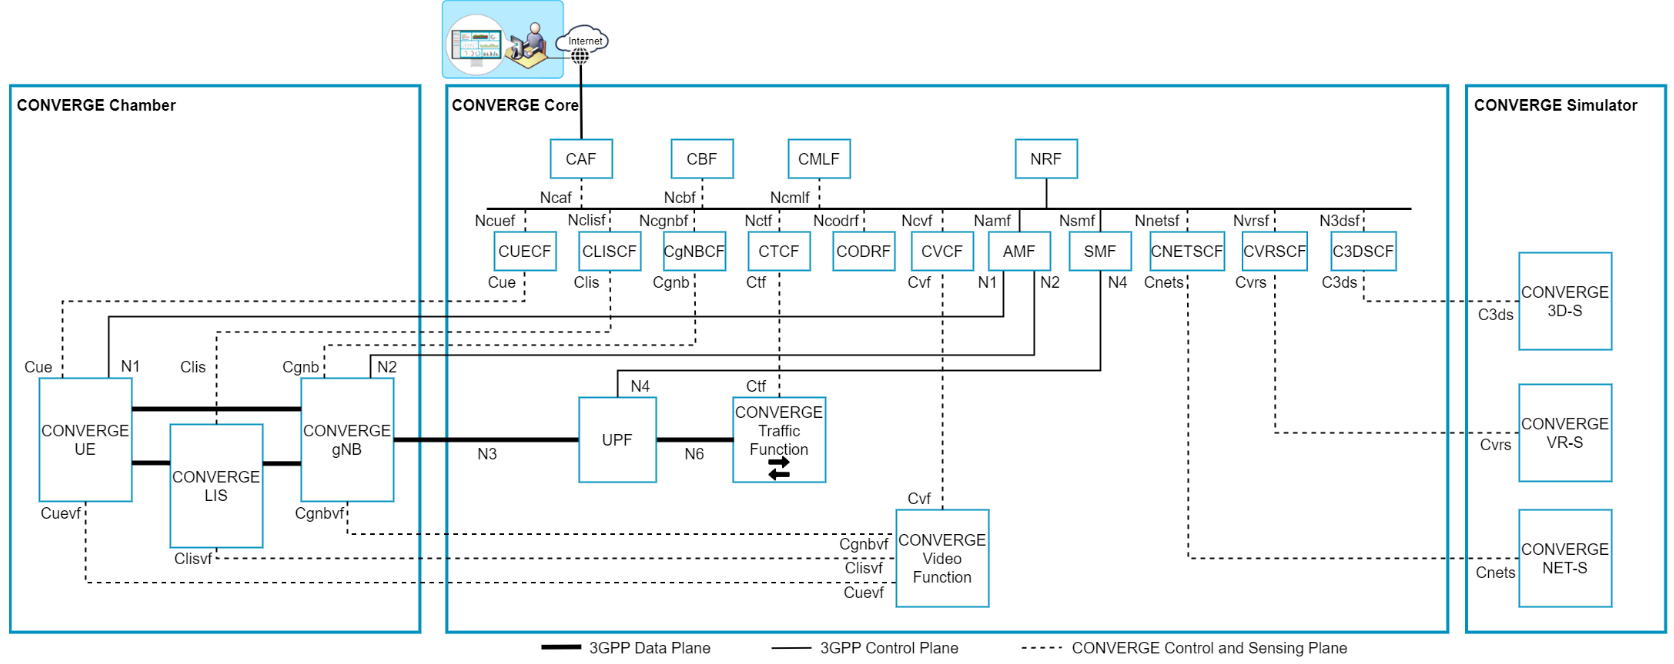
\includegraphics[width=1\linewidth]{figures/arch_converge}
    \caption[CONVERGE service-oriented architecture] {CONVERGE service-oriented architecture \cite{converge2023_specs}.}
    \label{fig:converge_arch}
\end{figure}

As detailed in~\cite{converge2023_specs}, the CONVERGE Video Control Function (CVCF) is responsible for managing the video cameras facilitating the utilization
of video tools within the chamber.
Moreover, it oversees and supports
vision models to extract information from the captured scenes.
The CONVERGE Video Control Function collaborates with the CONVERGE gNB through the CONVERGE dedicated gNB Control Function (CgNBCF).
This collaboration implies that the information from the video will be communicated to the CONVERGE gNB, enhancing its environmental awareness.
The CONVERGE Video Control Function, the gNB, and the Machine Learning models will
enhance connectivity and preemptively address challenges within the wireless environment.
By integrating advanced technologies and intelligent decision-making, the work
aims to contribute to the robustness and stability of wireless communications systems.


\section{Summary}\label{sec:Summary_SOA}
This chapter presents aspects of wireless communications, beginning with the evolution from 4G to 5G and the ambitious goals set for 6G.
It discusses the architecture of 5G, its components, and interfaces.
Moreover, it presents approaches to Radio Access Network (RAN) deployment, such as cRAN, vRAN, and the Open-RAN (O-RAN) architecture.

A substantial part of the chapter focuses on describing CV tools and applications.
It evaluates state-of-the-art detection and tracking models, focusing on the trade-off between speed, accuracy, and complexity.
The discussion extends to open-source tools in CV, emphasizing their relevance to wireless communications challenges.
The chapter also discusses the integration of CV into the broader context of wireless networks, providing a foundation for the subsequent exploration of video sensing in the field.

Additionally, the chapter presents related work to the problem posed in the introduction while presenting existing solutions leveraging video sensing.
Finally, the CONVERGE project is presented, as this dissertation leverages the project's architecture.
This chapter guides the current state of the convergence between CV and mobile networks, paving the way for a focused investigation in this dissertation.




